Esta seção descreve os materiais, métodos e decisões de projeto adotados no desenvolvimento do HormuzNet. São detalhados a arquitetura do sistema, os protocolos de comunicação implementados, os algoritmos distribuídos de tolerância a falhas e o ambiente de emulação utilizado para validação.

\subsection{Material e Método}
\label{sub:material_metodo}

O desenvolvimento e a avaliação experimental do HormuzNet basearam-se em computadores conectados via rede física Gigabit Ethernet no Laboratório LARSID da Universidade Estadual de Feira de Santana (UEFS). Os hosts executaram distribuições Linux (\textbf{Ubuntu} e \textbf{Mint}). O ambiente de software compreendeu:
\begin{itemize}
    \item \textbf{Linguagem de Programação:} Go (versão 1.21.2);
    \item \textbf{Motor de Contêineres:} Docker (versão 24.0.5);
    \item \textbf{Orquestrador:} Docker Compose (versão 2.20.2).
\end{itemize}

Foram testadas duas topologias: a \textbf{local}, com todos os contêineres em um único \textit{host} compartilhando rede virtual \textit{bridge}, e a \textbf{distribuída}, com a infraestrutura dividida entre duas máquinas físicas via LAN Gigabit. O cenário padrão instanciou \textbf{34 contêineres}: 9 \textit{brokers} (B1--B9), 6 drones autônomos, 18 sensores inteligentes (2 por setor) e 1 monitor tático. As métricas foram coletadas via chamadas \textit{curl} ao endpoint \texttt{/api/estado}, logs em tempo real pelo script \texttt{terminais.sh} e saída do comando \texttt{docker stats}.

\subsection{Arquitetura do Sistema}
\label{sub:arquitetura}

O HormuzNet afasta-se do modelo hierárquico centralizado do FarmNode, que dependia de um único \textit{broker} como SPOF. Em vez disso, adota um modelo \textbf{cliente-servidor em dois níveis}:
\begin{enumerate}
    \item[(i)] No primeiro nível, sensores e drones comportam-se como clientes dos \textit{brokers} de setor (servidores locais);
    \item[(ii)] No segundo nível, os \textit{brokers} formam entre si uma malha descentralizada P2P cooperativa.
\end{enumerate}

Essa topologia híbrida garante que mensagens de telemetria e coordenação circulem de forma redundante e resiliente pela malha geográfica. A Figura~\ref{fig:arquitetura} apresenta a organização dos componentes e a dinâmica de auto-organização da malha.

\begin{figure}[ht]
  \centering
  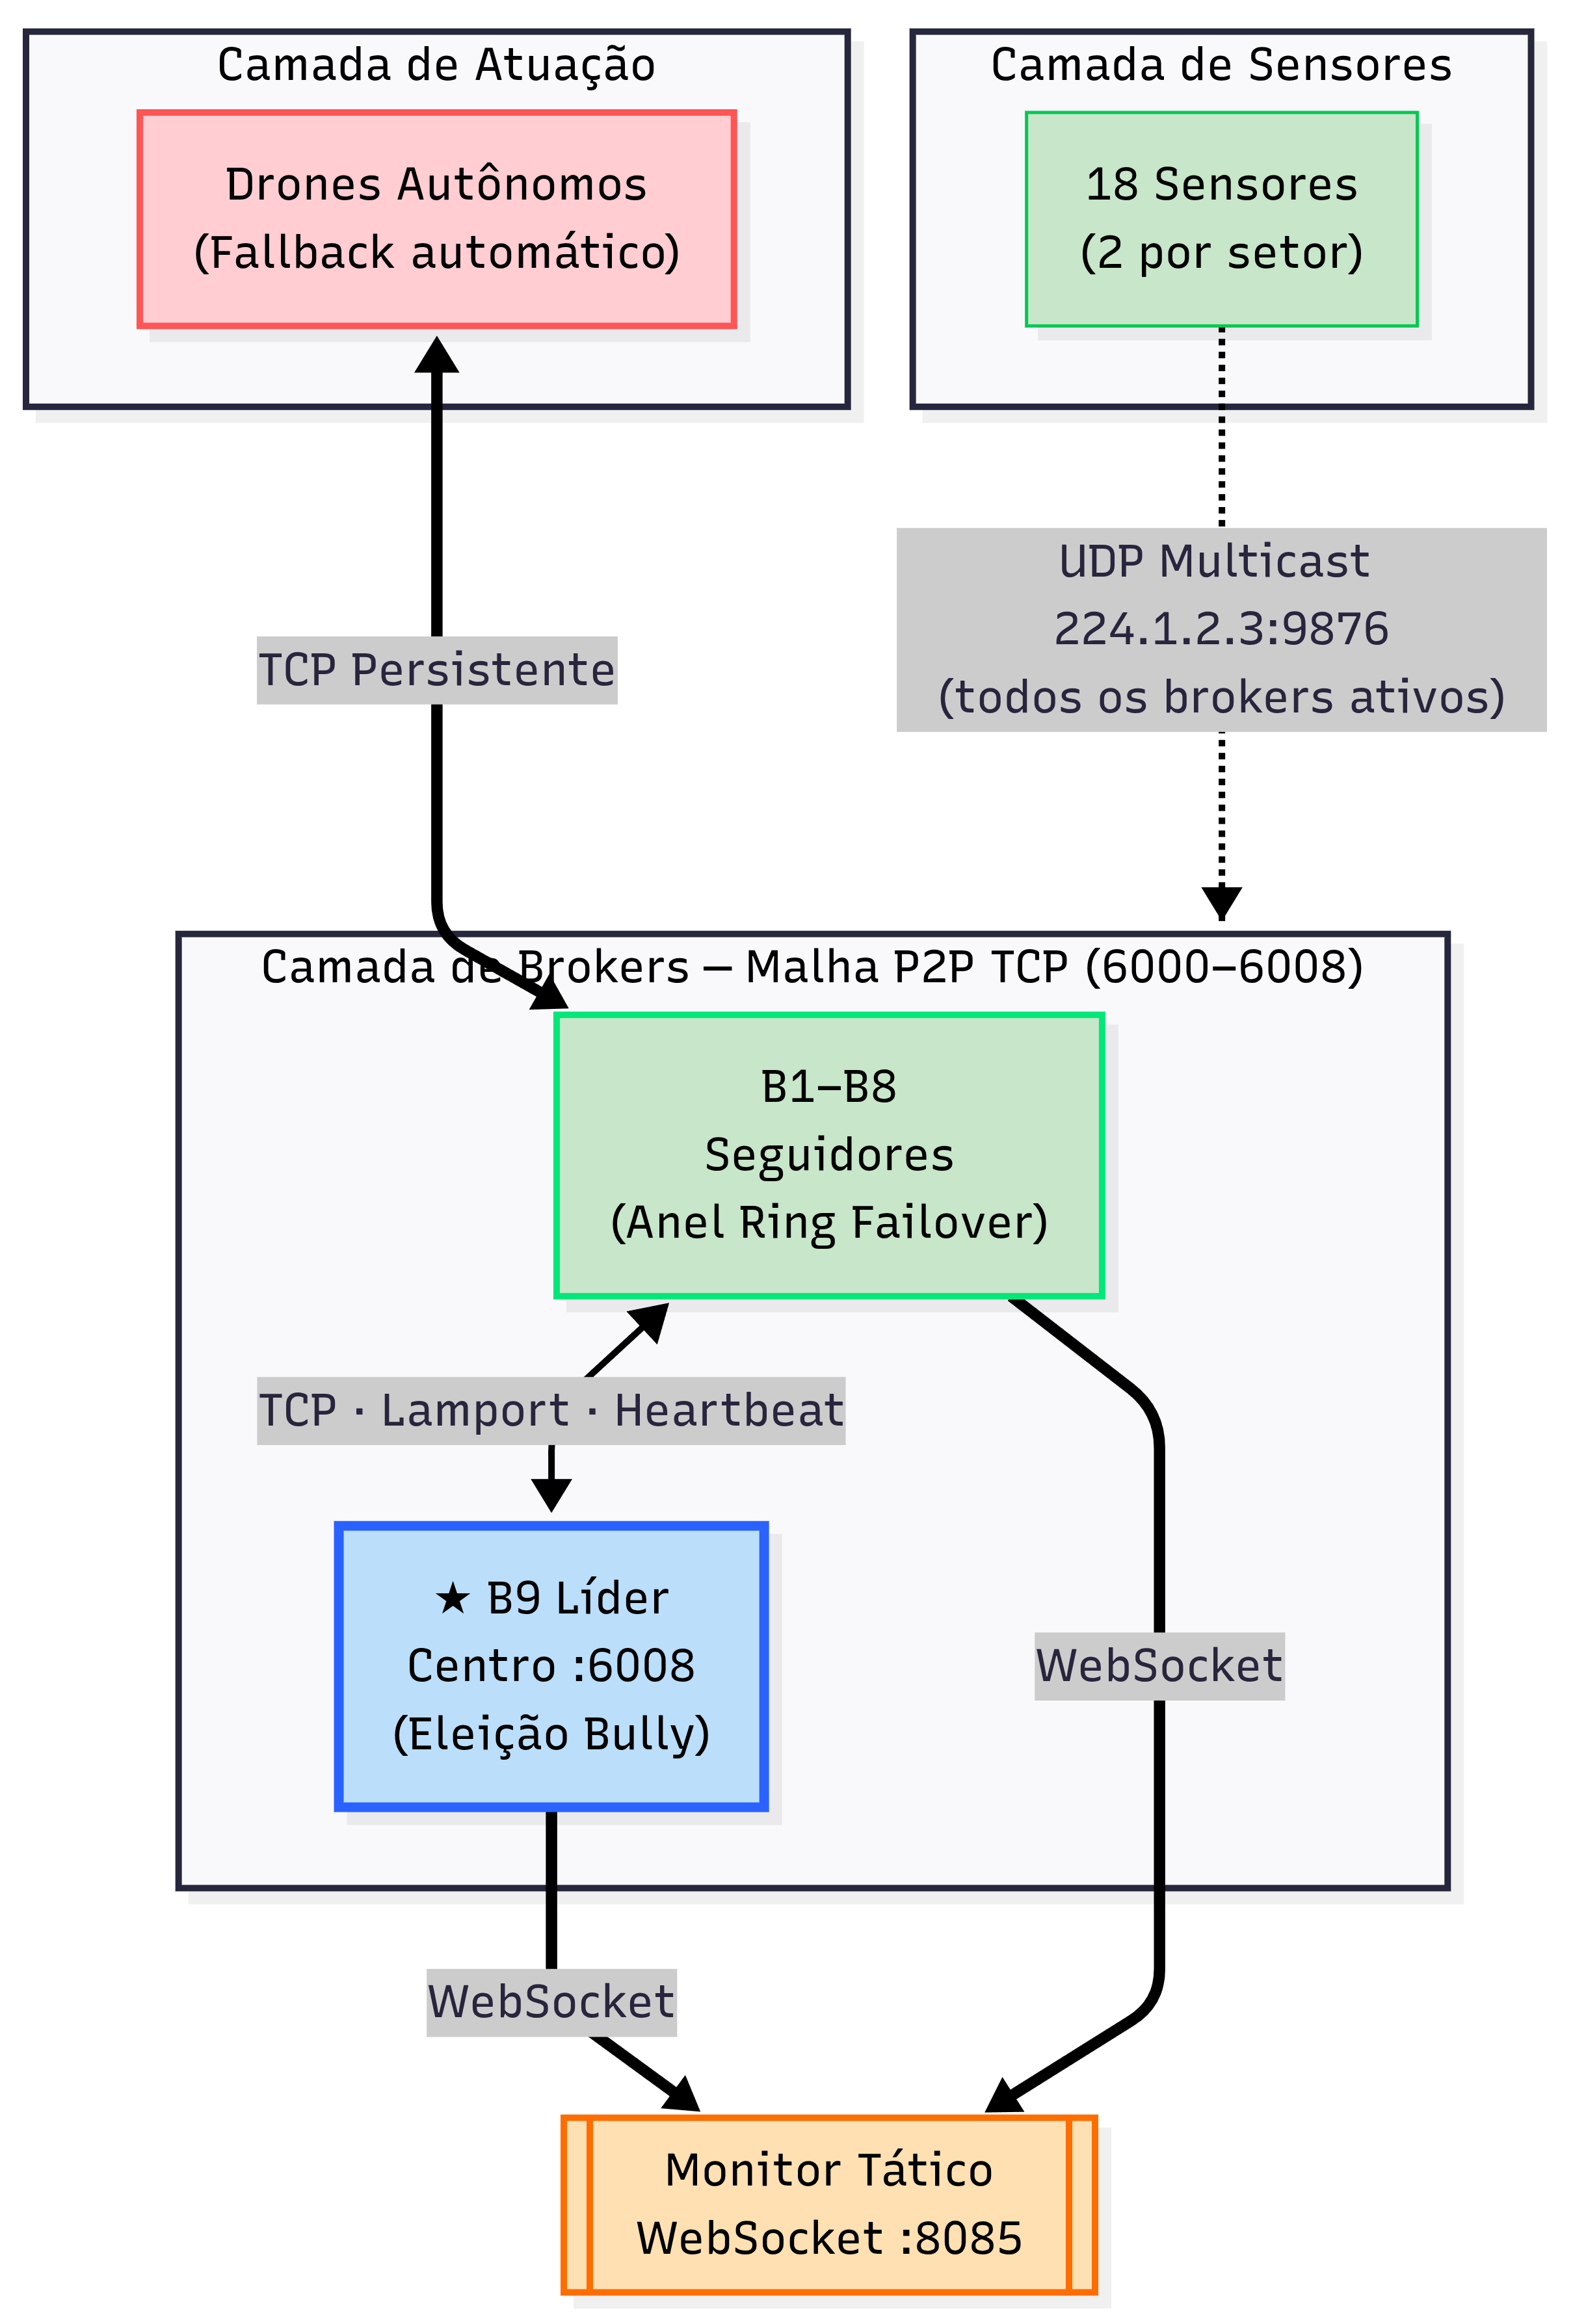
\includegraphics[width=0.45\textwidth]{figuras/arquitetura.png}
  \caption{Arquitetura descentralizada do HormuzNet com camadas de sensores, \textit{brokers} e drones. Fonte: Próprio Autor.}
  \label{fig:arquitetura}
\end{figure}

\subsection{Protocolo de Comunicação}
\label{sub:protocolo}

A troca de informações ocorre por meio de canais específicos detalhados na Tabela~\ref{tab:protocolo}.

\begin{table}[ht]
  \centering
  \sloppy
  \caption{Portas, protocolos e formatos dos canais de comunicação do HormuzNet. Fonte: Próprio Autor.}
  \label{tab:protocolo}
  \begin{tabular}{p{2.6cm}p{2.4cm}p{1.6cm}p{1.8cm}p{3.0cm}}
    \toprule
    \textbf{Fluxo} & \textbf{Protocolo} & \textbf{Porta} & \textbf{Formato} & \textbf{Propósito} \\
    \midrule
    Sensor $\to$ Broker & UDP/IP Multicast & 9876 & JSON UTF-8 & Telemetria e alertas \\
    Broker $\leftrightarrow$ Broker & TCP/IP P2P & 6000--6008 & JSON/linha & \textit{Gossip}, Lamport, Bully \\
    Drone $\leftrightarrow$ Broker & TCP/IP & 6000--6008 & JSON/linha & Registro e despacho \\
    Broker $\to$ Monitor & TCP/IP & 6000--6008 & JSON/linha & Logs e descoberta \\
    Monitor $\to$ Dashboard & WebSocket & 8085 & JSON \textit{frame} & \textit{Snapshot} tático \\
    \bottomrule
  \end{tabular}
\end{table}

Na telemetria, sensores publicam datagramas JSON no grupo \textit{multicast} \texttt{224.1.2.3:9876}; a delimitação de mensagem é o próprio tamanho do datagrama UDP/IP \cite{rfc768,rfc791}. Nos fluxos TCP/IP de coordenação, cada mensagem JSON é terminada por \texttt{\textbackslash{}n} e lida via \texttt{bufio.Scanner}.

\subsection{Descoberta, Filas e Concorrência}
\label{sub:descoberta_filas}

Ao iniciar, cada \textit{broker} seguidor conecta-se ao líder e recebe a lista de membros ativos (\texttt{PEER\_LIST}), estabelecendo suas conexões TCP P2P dinamicamente. Drones registram-se no \textit{broker} de seu setor e, em caso de falha deste, executam \textit{fallback} automático para o vizinho seguinte na lista de setores. Cada \textit{broker} mantém um \textit{heap} binário \textit{thread-safe} com capacidade para até 262.144 ocorrências; o despacho seleciona o drone disponível de menor distância cartesiana ao incidente, emite o comando \texttt{DESPACHAR\_DRONE} via TCP e propaga a remoção do evento por \textit{broadcast} à malha. A concorrência é gerenciada com \textit{goroutines} por \textit{socket} e \textit{mutexes} por recurso, com \textit{timeout} de escrita de 2\,s para prevenir bloqueios.

\subsection{Confiabilidade: \textit{Heartbeat} e \textit{Ring Failover}}
\label{sub:confiabilidade}

\textit{Brokers} emitem \textit{heartbeats} a cada 5\,s para seus vizinhos P2P. Após 15\,s sem resposta, o nó é marcado como inativo: o vizinho anterior no anel lógico assume o setor (\textit{Ring Failover}), os drones do \textit{broker} inativo reconectam-se por \textit{backoff} ao próximo vizinho disponível e, caso o líder tenha falhado, os seguidores iniciam imediatamente o algoritmo Bully para eleição de novo coordenador.

\subsection{Emulação e Testes}
\label{sub:emulacao}

O ambiente de emulação injeta distúrbios realísticos de forma contínua: ocorrências permanecem na fila sob \textit{aging} de 30\,s, com incremento de criticidade a cada ciclo sem atendimento; drones em patrulha entram em alerta de ociosidade após 60\,s sem missão; e cada drone possui 10\% de probabilidade de ser abatido em trânsito, forçando o \textit{broker} a registrar a perda e re-enfileirar a ocorrência na malha.
